\chapter{文件系统}

\section{实验目的}
  \begin{enumerate}
    \item 了解文件系统的基本概念和作用。
    \item 了解普通磁盘的基本结构和读写方式。
    \item 掌握并实现文件系统的基本操作。
    \item 了解微内核的基本设计思想和结构。
  \end{enumerate}

\section{背景知识}

\subsection{文件系统}

计算机的文件系统是一种存储和组织计算机数据的方法,它使得对其访问和查找变得容易,文件系统使用文件和树形目录
的抽象逻辑概念代替了硬盘和光盘等物理设备使用数据块的概念,用户使用文件系统来保存数据不必关心数据实际保存在
硬盘(或者光盘)的地址为多少的数据块上,只需要记住这个文件的所属目录和文件名。在写入新数据之前,用户不必关
心硬盘上的那个块地址没有被使用,硬盘上的存储空间管理(分配和释放)功能由文件系统自动完成,用户只需要记住数
据被写入到了哪个文件中。

文件系统通常使用硬盘和光盘这样的存储设备,并维护文件在设备中的物理位置。但是,实际上文件系统也可能仅仅是一
种访问数据的界面而已,实际的数据是通过网络协议(如NFS、SMB、9P等)提供的或者内存上,甚至可能根本没有对应
的文件(如 proc文件系统)。

\begin{thinking}\label{think-proc}
查阅资料,了解Linux/Unix的 /proc 文件系统是什么?有什么作用?Windows操作系统又是如何实现这些功能的?proc
文件系统这样的设计有什么好处?
\end{thinking}

\subsection{磁盘}

接下来简单介绍一下与磁盘相关的基本知识。磁盘相关的几个基本概念:

\begin{enumerate}
  \item 扇区(Sector):磁盘盘片被划分成很多扇形的区域,叫做扇区。扇区是磁盘执行读写操作的单位,一般是512字节。
  扇区的大小是一个磁盘的硬件属性。
  \item 磁道(track): 盘片上以盘片中心为圆心,不同半径的同心圆。
  \item 柱面(cylinder):硬盘中,不同盘片相同半径的磁道所组成的圆柱。
  \item 磁头(head):每个磁盘有两个面,每个面都有一个磁头。当对磁盘进行读写操作时,磁头在盘片上快速移动。
\end{enumerate}

典型的磁盘的基本结构如图\ref{lab5-pic-1}所示:

\begin{figure}[htbp]
  \centering
  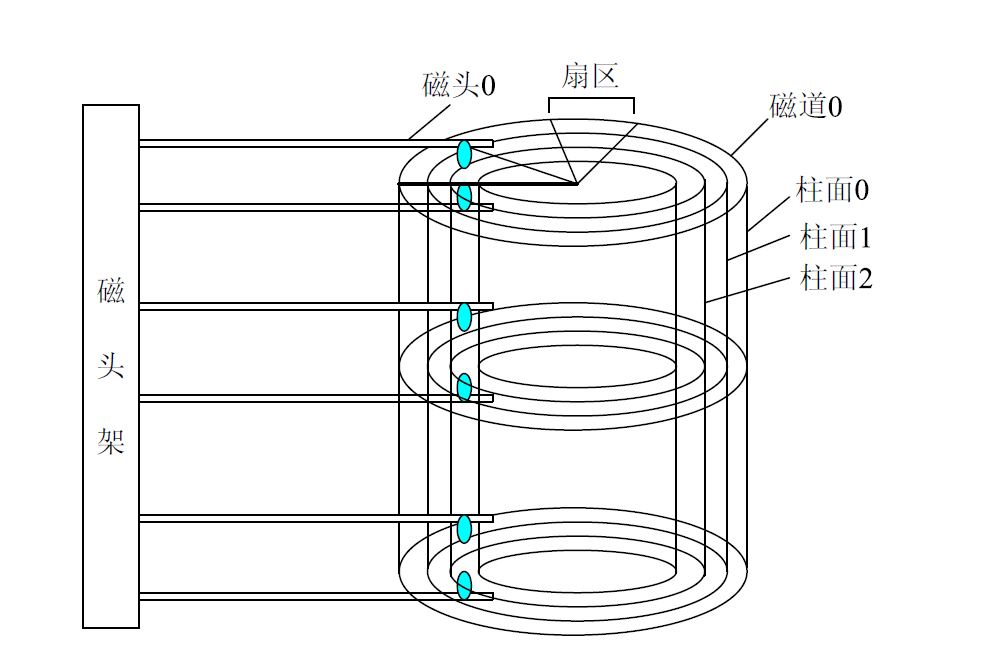
\includegraphics[width=12cm]{lab5-pic-1}
  \caption{磁盘结构示意图}\label{lab5-pic-1}
\end{figure}

\section{IDE磁盘}

\begin{note}
IDE 的英文全称为“Integrated Drive Electronics”,即“电子集成驱动器”,是目前最主流的硬盘接口, 也是光储类
设备的主要接口。IDE接口,也称之为ATA接口。
\end{note}

在我们的操作系统实验中,我们使用的 Gxemul 模拟器提供了一个 IDE 
仿真设备,我们需要此基础上实现我们的文件系统,接下来,我们将了解一些读写 IDE 磁盘的基础知识。

\subsection{内存映射I/O}

在第二次试验中,我们已经了解了MIPS存储器地址映射的基本内容。几乎每一种外设都是通过读写设备上的寄存器来进行数据通信,
外设寄存器也称为\textbf{I/O端口},我们使用I/O端口来访问I/O设备。外设寄存器通常包括控制寄存器、状态寄存器和
数据寄存器。这些硬件I/O寄存器被映射到指定的内存空间,例如,在 Gxemul 中,console 设备被映射到
\mintinline{c}|0x10000000|,simulated IDE disk被映射到 0x13000000,等等。更详细的关于 Gxemul 的仿真
设备的说明,可以参考\href{http://gxemul.sourceforge.net/gxemul-stable/doc/experiments.html}{Gxemul
Experimental Devices}。

驱动程序访问的是IO空间,与一般我们说的内存空间是不同的。外设的IO空间地址是系统启动后才知道,CPU通常并没有为这些已
知的外设I/O内存资源的物理地址预定义虚拟地址范围,所以驱动程序并不能直接通过物理地址访问I/O内存资源,而\textbf{必须
将它们映射到内核虚地址空间内然后才能根据映射所得到的核心虚地址范围},通过访存指令访问这些I/O内存资源。

咱们的操作系统内核中,将物理内存转换为内核虚拟地址,可以使用\mintinline{c}|KADDR|宏,也就是将物理地址加上
\mintinline{c}|ULIM|的值(\mintinline{c}|0x80000000|)。

例如,Gxemul 提供的 console 设备的地址:0x10000000,设备寄存器映射如表\ref{lab5-table-console-mem-map}所示:

\begin{table}[htbp]
\caption{Gexmul Console 内存映射}\label{lab5-table-console-mem-map}
\centering
\begin{tabular}{|c|l|}
  \hline
    Offset & Effect \\
  \hline
  \multirow{2}{*}{0x00} & Read: getchar() (non-blocking; returns 0 if no char was available) \\
  \cline{2-2}
    & Write: putchar(ch) \\
  \hline
    \multirow{2}{*}{0x10} & Read or write: halt() \\
  \cline{2-2}
    & (Useful for exiting the emulator.) \\
  \hline
\end{tabular}
\end{table}

现在,我们通过往内存的 (0x10000000+0x80000000) 地址写入字符,就能在 shell 中看到对应的输出。
\mintinline{c}|drivers/gxconsole/console.c|中的\mintinline{c}|printcharc|函数的实现如下所示:

\begin{minted}[linenos]{c}
void printcharc(char ch)
{
  *((volatile unsigned char *) PUTCHAR_ADDRESS) = ch;
}
\end{minted}

\subsection{IDE磁盘操作}

磁盘的访问跟 Console 类似,也是将要用到的磁盘设备的 I/O 寄存器映射到制定的虚存地址。前文中我们提到过,扇区(Sector)
是磁盘读写的基本单位,Gxemul 也提供了对扇区进行操作的基本方法。

Gexmul 提供的 Simulated IDE disk 的地址是 0x13000000,I/O寄存器相对于 \mintinline{c}|0x13000000| 的偏
移和对应的功能如表\ref{lab5-table-disk-mem-map}所示:

\begin{table}[htbp]
\caption{Gexmul IDE disk I/O 寄存器映射}\label{lab5-table-disk-mem-map}
\centering
\begin{tabular}{|c|p{12cm}|}
  \hline
    Offset & Effect \\
  \hline
    0x0000 & Write: Set the offset (in bytes) from the beginning of the disk image. This offset will be used for the next read/write operation. \\
  \hline
    0x0008 & Write: Set the high 32 bits of the offset (in bytes). (*) \\
  \hline
    0x0010 & Write: Select the IDE ID to be used in the next read/write operation. \\
  \hline
    0x0020 & Write: Start a read or write operation. (Writing 0 means a Read operation, a 1 means a Write operation.) \\
  \hline
    0x0030 & Read: Get status of the last operation. (Status 0 means failure, non-zero means success.) \\
  \hline
    0x4000-0x41ff  &  Read/Write: 512 bytes data buffer. \\
  \hline
\end{tabular}
\end{table}

通过对\mintinline{c}|printcharc| 函数的实现的分析,我们已经掌握了I/O操作的基本方法,那么,读写 IDE disk 
的相关代码也就不难理解了。以从硬盘上读取一些 Sectors 为例,涉及到的函数有 \mintinline{c}|fs/ide.c| 中的 
\mintinline{c}|ide_read| 函数和 \mintinline{c}|fs/ide_asm.S|中的 \mintinline{c}|read_sector| 函数。
具体代码如下:

\mintinline{c}|ide_read| 函数:

\begin{minted}[linenos]{c}
extern int read_sector(int diskno, int offset);

void ide_read(u_int diskno, u_int secno, void *dst, u_int nsecs)
{
    // 0x200: the size of a sector: 512 bytes.
    int offset_begin = secno * 0x200;
    int offset_end = offset_begin + nsecs * 0x200;
    int offset = 0;

    while (offset_begin + offset < offset_end) {
        if (read_sector(diskno, offset_begin + offset)) {
            // copy data from disk buffer(512 bytes, a sector) to destination array.
            user_bcopy((void *)0x93004000, dst + offset, 0x200);
            offset += 0x200;
        } else {
            // error occurred, then panic.
            user_panic("disk I/O error");
        }
    }
}
\end{minted}

\mintinline{c}|read_sector| 函数:

\begin{minted}[linenos]{asm}
// read sector at specified offset from the beginning of the disk image.
LEAF(read_sector)
    sw  a0, 0x93000010  // select the IDE id.
    sw  a1, 0x93000000  // offset.
    li  t0, 0
    sb  t0, 0x93000020  // start read.
    lw  v0, 0x93000030
    nop
    jr  ra
    nop
END(read_sector)
\end{minted}

我们来分析这两段代码。当需要从磁盘的指定位置读取一个 sector 时,需要调用 \mintinline{c}|read_sector|
函数来将磁盘中对应sector 的数据读到设备缓冲区中。\textbf{所有的地址操作都需要将物理地址转换成内核虚拟地址}。
根据Gxemul提供的与 ide disk 相关的数据表格,首先,设置 IDE disk 的 ID,从
\mintinline{c}|read_sector| 函数的声明 \mintinline{c}|extern int read_sector(int diskno, int offset);|
中可以看出,diskno 是第一个参数,对应的就是 \$a0 寄存器的值,因此,将其写入到 0x93000010 处,这样就表示
我们将使用编号为 \$a0 的磁盘。我们的试验中,只使用了一块 simulated IDE disk, 因此,这个值应该为 0。
接下来,将相对于磁盘起始位置的 offset 写入到 0x93000000 位置,表示在距离磁盘起始处 offset 的位置开始
进行磁盘操作。然后,根据 Gxemul 的 data sheet,向内存 0x93000020 处写入 0 来开始读磁盘(如果是写磁盘,则写
入 1)。
最后,将磁盘操作的状态码放入 \$v0 中,作为结果返回给 \mintinline{c}|ide_read| 函数。
在 \mintinline{c}|ide_read| 函数中,我们通过判断 \mintinline{c}|read_sector| 函数的返回值,
就可以知道读取磁盘的操作是否成功。如果成功,将这个 sector 的数据(512 bytes) 从设备缓冲区 (0x4000-0x41ff) 
中拷贝到目的位置(此处的 \mintinline{c}|void *dst|)。至此,我们就完成了对磁盘的读操作。

写磁盘的操作与读磁盘的一个区别在于写磁盘需要先将要写入对应 sector 的 512 bytes 的数据放入设备缓冲中,然后向地
址 0x93000020处写入 1 来启动操作,并从 0x93000030 处获取写磁盘操作的返回值。

\begin{exercise}
参考 \mintinline{c}|ide_read| 函数和 \mintinline{c}|read_sector| 函数的实现方式,实现 fs/ide.c 中
的 \mintinline{c}|ide_write| 函数,以及 fs/ide\_asm.S 中的 \mintinline{c}|write_sector| 函数,
实现对磁盘的写操作。
\end{exercise}

\section{文件系统结构}

\begin{note}
Unix/Linux操作系统一般将磁盘分成两个区域:inode 区域和 data 区域。inode 区域用来保存文件的状态属性,
以及指向数据块的指针。data 区域用来存放文件的内容和目录的元信息(包含的文件)。我们实验使用的操作系统内核的文件系统
也采用类似的设计。
\end{note}

\subsection{磁盘布局}

磁盘空间的基本布局如图\ref{lab5-pic-2}所示。

\begin{figure}[htbp]
  \centering
  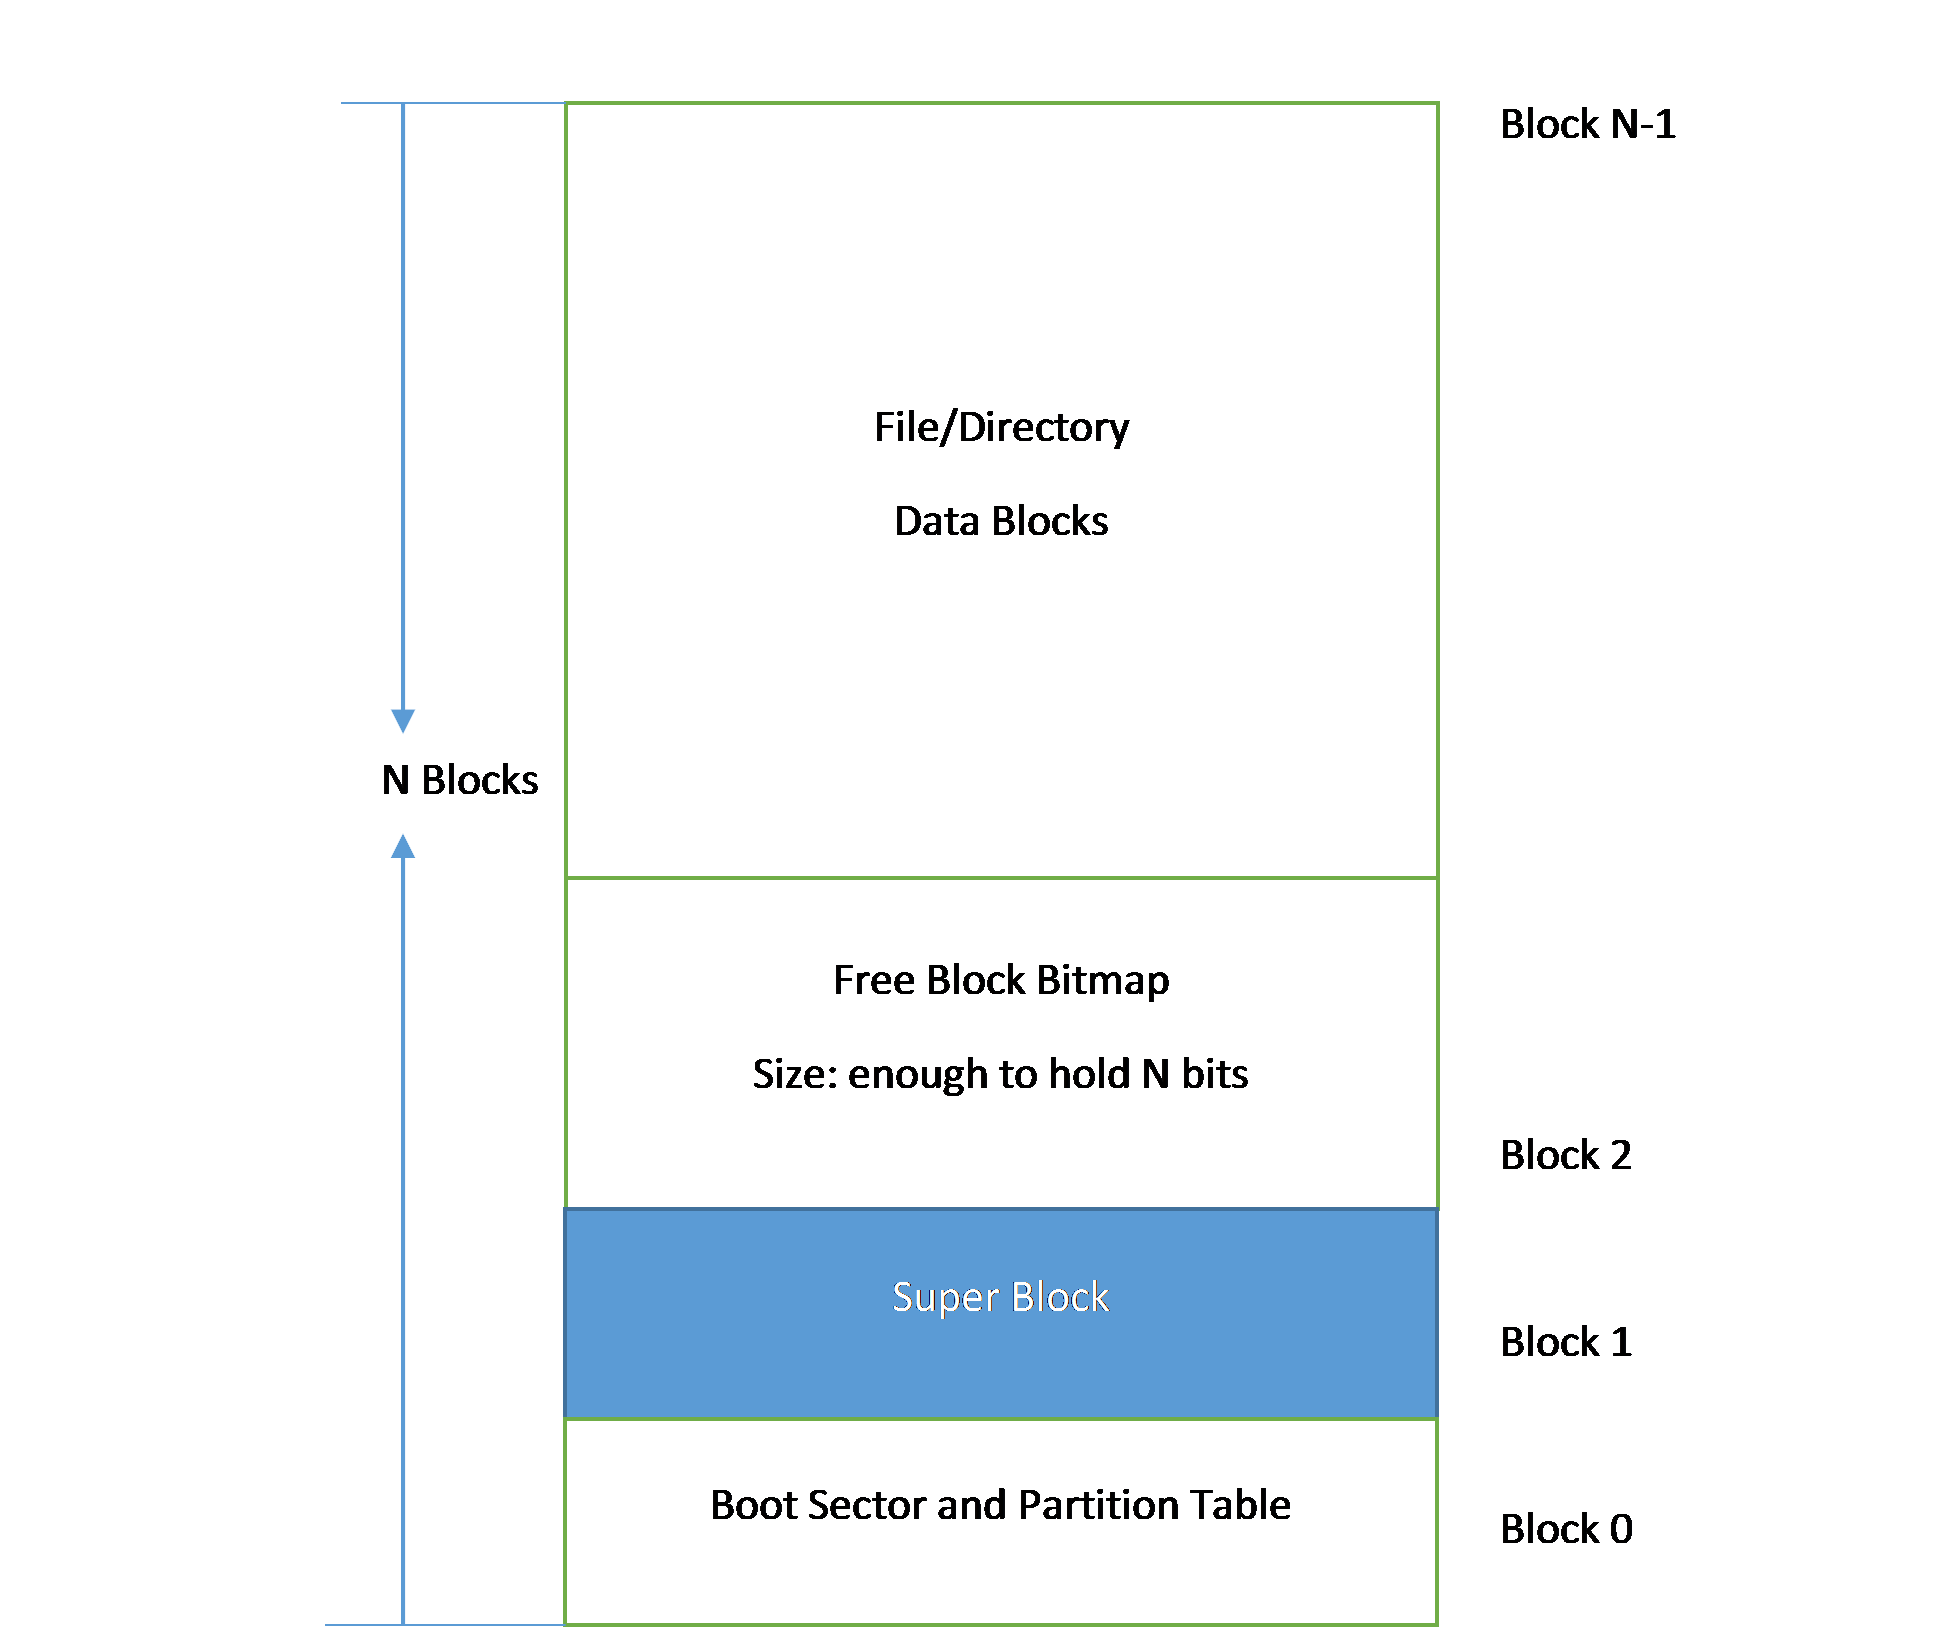
\includegraphics[width=12cm]{lab5-pic-2}
  \caption{磁盘空间布局示意图}\label{lab5-pic-2}
\end{figure}

从图中可以看到磁盘最开始的一个扇区(512字节)被当成是启动扇区和分区表使用。接下来的一个扇区用作
超级块(Super Block),用来描述文件系统的基本信息,如 Magic Number,磁盘大小,以及根目录的位置。

\begin{note}
在真真实的文件系统中,一般会维护多个超级块,通过复制分散到不同的磁盘分区中,以防止超级块的损坏造成整个磁盘
无法使用。
\end{note}

我们的操作系统中超级块的结构:

\begin{minted}[linenos]{c}
struct Super {
    u_int s_magic;      // Magic number: FS_MAGIC
    u_int s_nblocks;    // Total number of blocks on disk
    struct File s_root; // Root directory node
};
\end{minted}

超级块的内容包括一个 magic number,磁盘中 block 的个数,以及根目录。

操作系统有两种常用的方式来管理资源:空闲链表和位图。在第二次试验和第三次试验中,我们使用了空闲链表来管理
空闲内存资源和进程控制块。在文件系统中,我们将使用位图(Bitmap)法来管理空闲的磁盘资源。具体来说,我们使用
一个二进制位来表示磁盘上的一个块(Block)是否使用。

接下来,我们来学习如何使用 bitmap 来标识磁盘中的所有块的使用情况。

fs/fsformat 用于将多个文件按照我们的内核所定义的文件系统写入到磁盘镜像中。在写入文件之前,我们将所有的块
全部都标为空闲块:

\begin{minted}[linenos]{c}
    nbitblock = (nblock + BIT2BLK - 1) / BIT2BLK;
    for(i = 0; i < nbitblock; ++i) {
        memset(disk[2+i].data, 0xff, nblock/8);
    }
    if(nblock != nbitblock * BY2BLK) {
        diff = nblock % BY2BLK / 8;
        memset(disk[2+(nbitblock-1)].data+diff, 0x00, BY2BLK - diff);
    }
\end{minted}

nbitblock 表示要记录整个磁盘上所有块的使用信息,我们需要多少个块来存储位图。紧接着,我们将所有位图块的每一位都标记为
0x1,表示这一块磁盘处于空闲状态。需要格外注意的是,如果 bitmap 还有剩余,我们不能将最后一块位图块靠后的一部分内容标记为
空闲,因为这些位所对应的磁盘块并不存在,不可被使用。因此,在 fs/fsformat.c 中的 \mintinline{c}|init_disk|
函数中,在将所有的位图块都置为 0x1 之后,还需要根据实际情况,将多出来的位图标记为 0x0。

在我们的操作系统内核中,文件系统也需要根据 bitmap 来判断和标记磁盘的使用情况。fs/fs.c 中的 \mintinline{c}|block_is_free|
函数就用来通过 bitmap 中的特定位来判断指定的磁盘块是否被占用。

\begin{minted}[linenos]{c}
int block_is_free(u_int blockno)
{
    if (super == 0 || blockno >= super->s_nblocks) {
        return 0;
    }
    if (bitmap[blockno / 32] & (1 << (blockno % 32))) {
        return 1;
    }
    return 0;
}
\end{minted}

\begin{exercise}
文件系统需要负责维护磁盘块的申请和释放,在回收一个磁盘块时,需要更改 bitmap 中的标志位。如果要将一个磁盘块设置为 free,
只需要将 bitmap 中对应的 bit 的值设置为 0x0 即可。请完成 fs/fs.c 中的 \mintinline{c}|free_block| 函数,
实现这一功能。同时思考为什么参数 \mintinline{c}|blockno| 的值不能为 0 ?

\begin{minted}[linenos]{c}
// Overview:
//  Mark a block as free in the bitmap.
void
free_block(u_int blockno)
{
    // Step 1: Check if the parameter `blockno` is valid (`blockno` can't be zero). 

    // Step 2: Update the flag bit in bitmap.

}
\end{minted}

\end{exercise}

\subsection{块缓存}

块缓存指的是借助虚拟内存来实现磁盘块缓存的设计。我们实验使用的内核中,文件系统是一个用户进程,一个进程可以拥有 4G 
的虚拟内存空间,将 \mintinline{c}|DISKMAP| 到 \mintinline{c}|DISKMAP+DISKMAX| 这一段虚存地址空间
(0x10000000-0xcffffff) 作为缓冲区,当磁盘读入内存时,用来映射相关的页。\mintinline{c}|DISKMAP| 和
\mintinline{c}|DISKMAX| 的值定义在 fs/fs.h 中:

\begin{minted}[linenos]{c}
#define DISKMAP   0x10000000
#define DISKMAX   0xc0000000
\end{minted}

\begin{thinking}\label{think-disksize}
请思考,在满足磁盘块缓存的设计的前提下,我们实验使用的内核支持的最大磁盘大小是多少?
\end{thinking}

为了建立起磁盘地址空间和进程虚存地址空间之间的缓存映射,我们采用这样一种设计:结构如图\ref{lab5-pic-4}。

\begin{figure}[htbp]
  \centering
  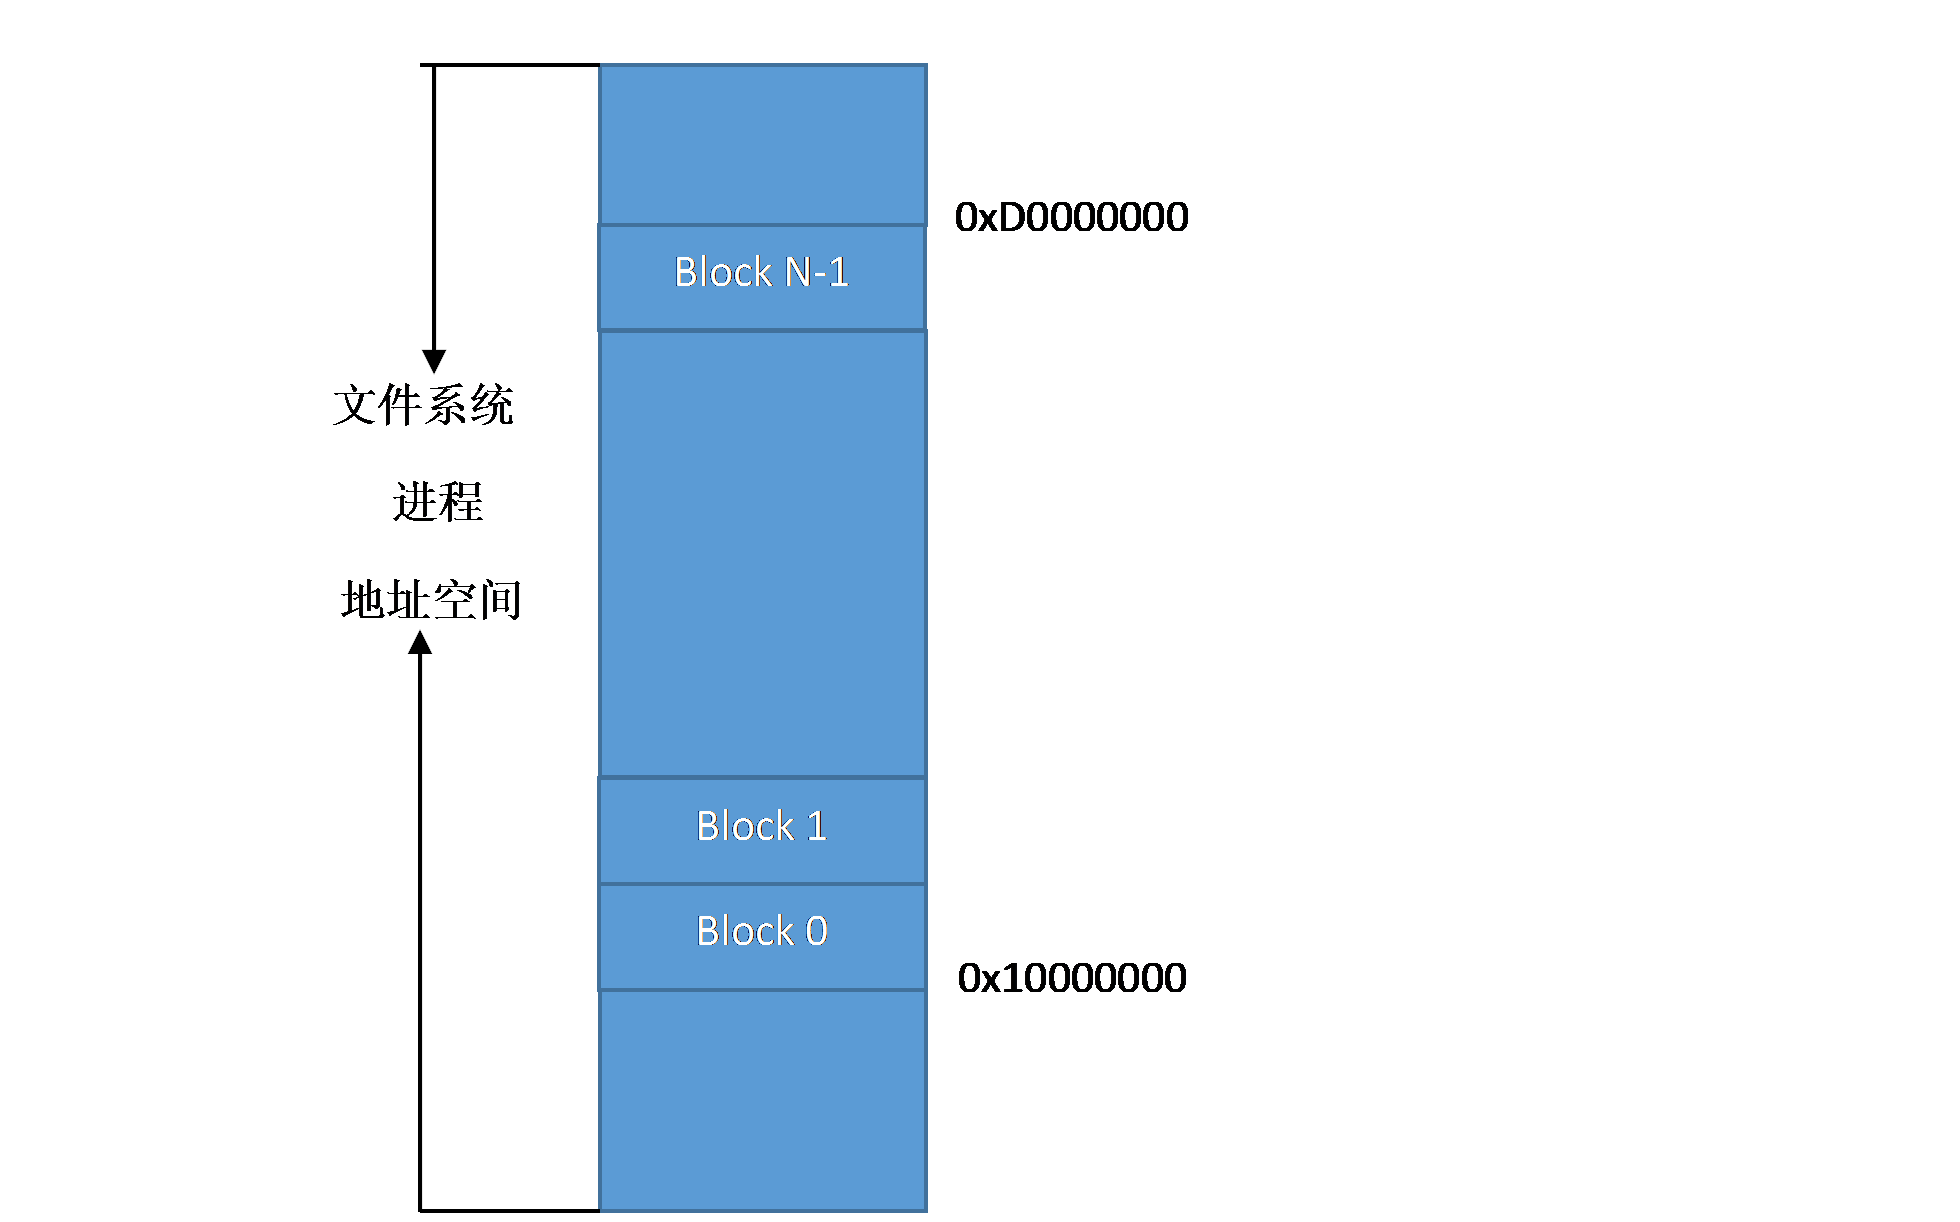
\includegraphics[width=12cm]{lab5-pic-4}
  \caption{块缓存示意图}\label{lab5-pic-4}
\end{figure}

\begin{exercise}
fs/fs.c 中的 diskaddr 函数用来计算指定磁盘块对应的虚存地址。完成 \mintinline{c}|diskaddr| 函数,根据
一个块的序号(block number),计算这一磁盘块对应的 512 bytes 虚存的起始地址。(提示:fs/fs.h 中的宏
\mintinline{c}|DISKMAP| 和 \mintinline{c}|DISKMAX| 定义了磁盘映射虚存的地址空间)。
\end{exercise}

当我们把一个磁盘块(block)中的内容载入到内存中时,我们需要为之分配对应的物理内存,当结束使用这一磁盘块时,需要释放对应的
物理内存以回收操作系统资源。fs/fs.c 中的 \mintinline{c}|map_block| 函数和 \mintinline{c}|unmap_block| 函
数实现了这一功能。

\begin{exercise}
实现 \mintinline{c}|map_block| 函数,检查指定的磁盘块是否已经映射到内存,如果没有,分配一页内存来保存磁盘上的数据。对应地,
完成 \mintinline{c}|unmap_block| 函数,用于接触磁盘块和物理内存之间的映射关系,回收内存。(提示:注意磁盘虚拟内存地址空间
和磁盘块之间的对应关系)。
\end{exercise}

\mintinline{c}|read_block| 函数和 \mintinline{c}|write_block| 函数用于读写磁盘块。\mintinline{c}|read_block|
函数将指定编号的磁盘块都入到内存中,首先检查这块磁盘块是否已经在内存中,如果不在,先分配一页物理内存,然后调用
\mintinline{c}|ide_read| 函数来读取磁盘上的数据到对应的虚存地址处。

\subsection{文件系统详细结构}

在操作系统的学习中,我们多次提到,操作系统要想管理一类资源,就得有相应的数据结构。我们使用文件控制块来描述和管理文件。
文件在磁盘上的组织形式如图\ref{lab5-pic-3}所示:

\begin{figure}[htbp]
  \centering
  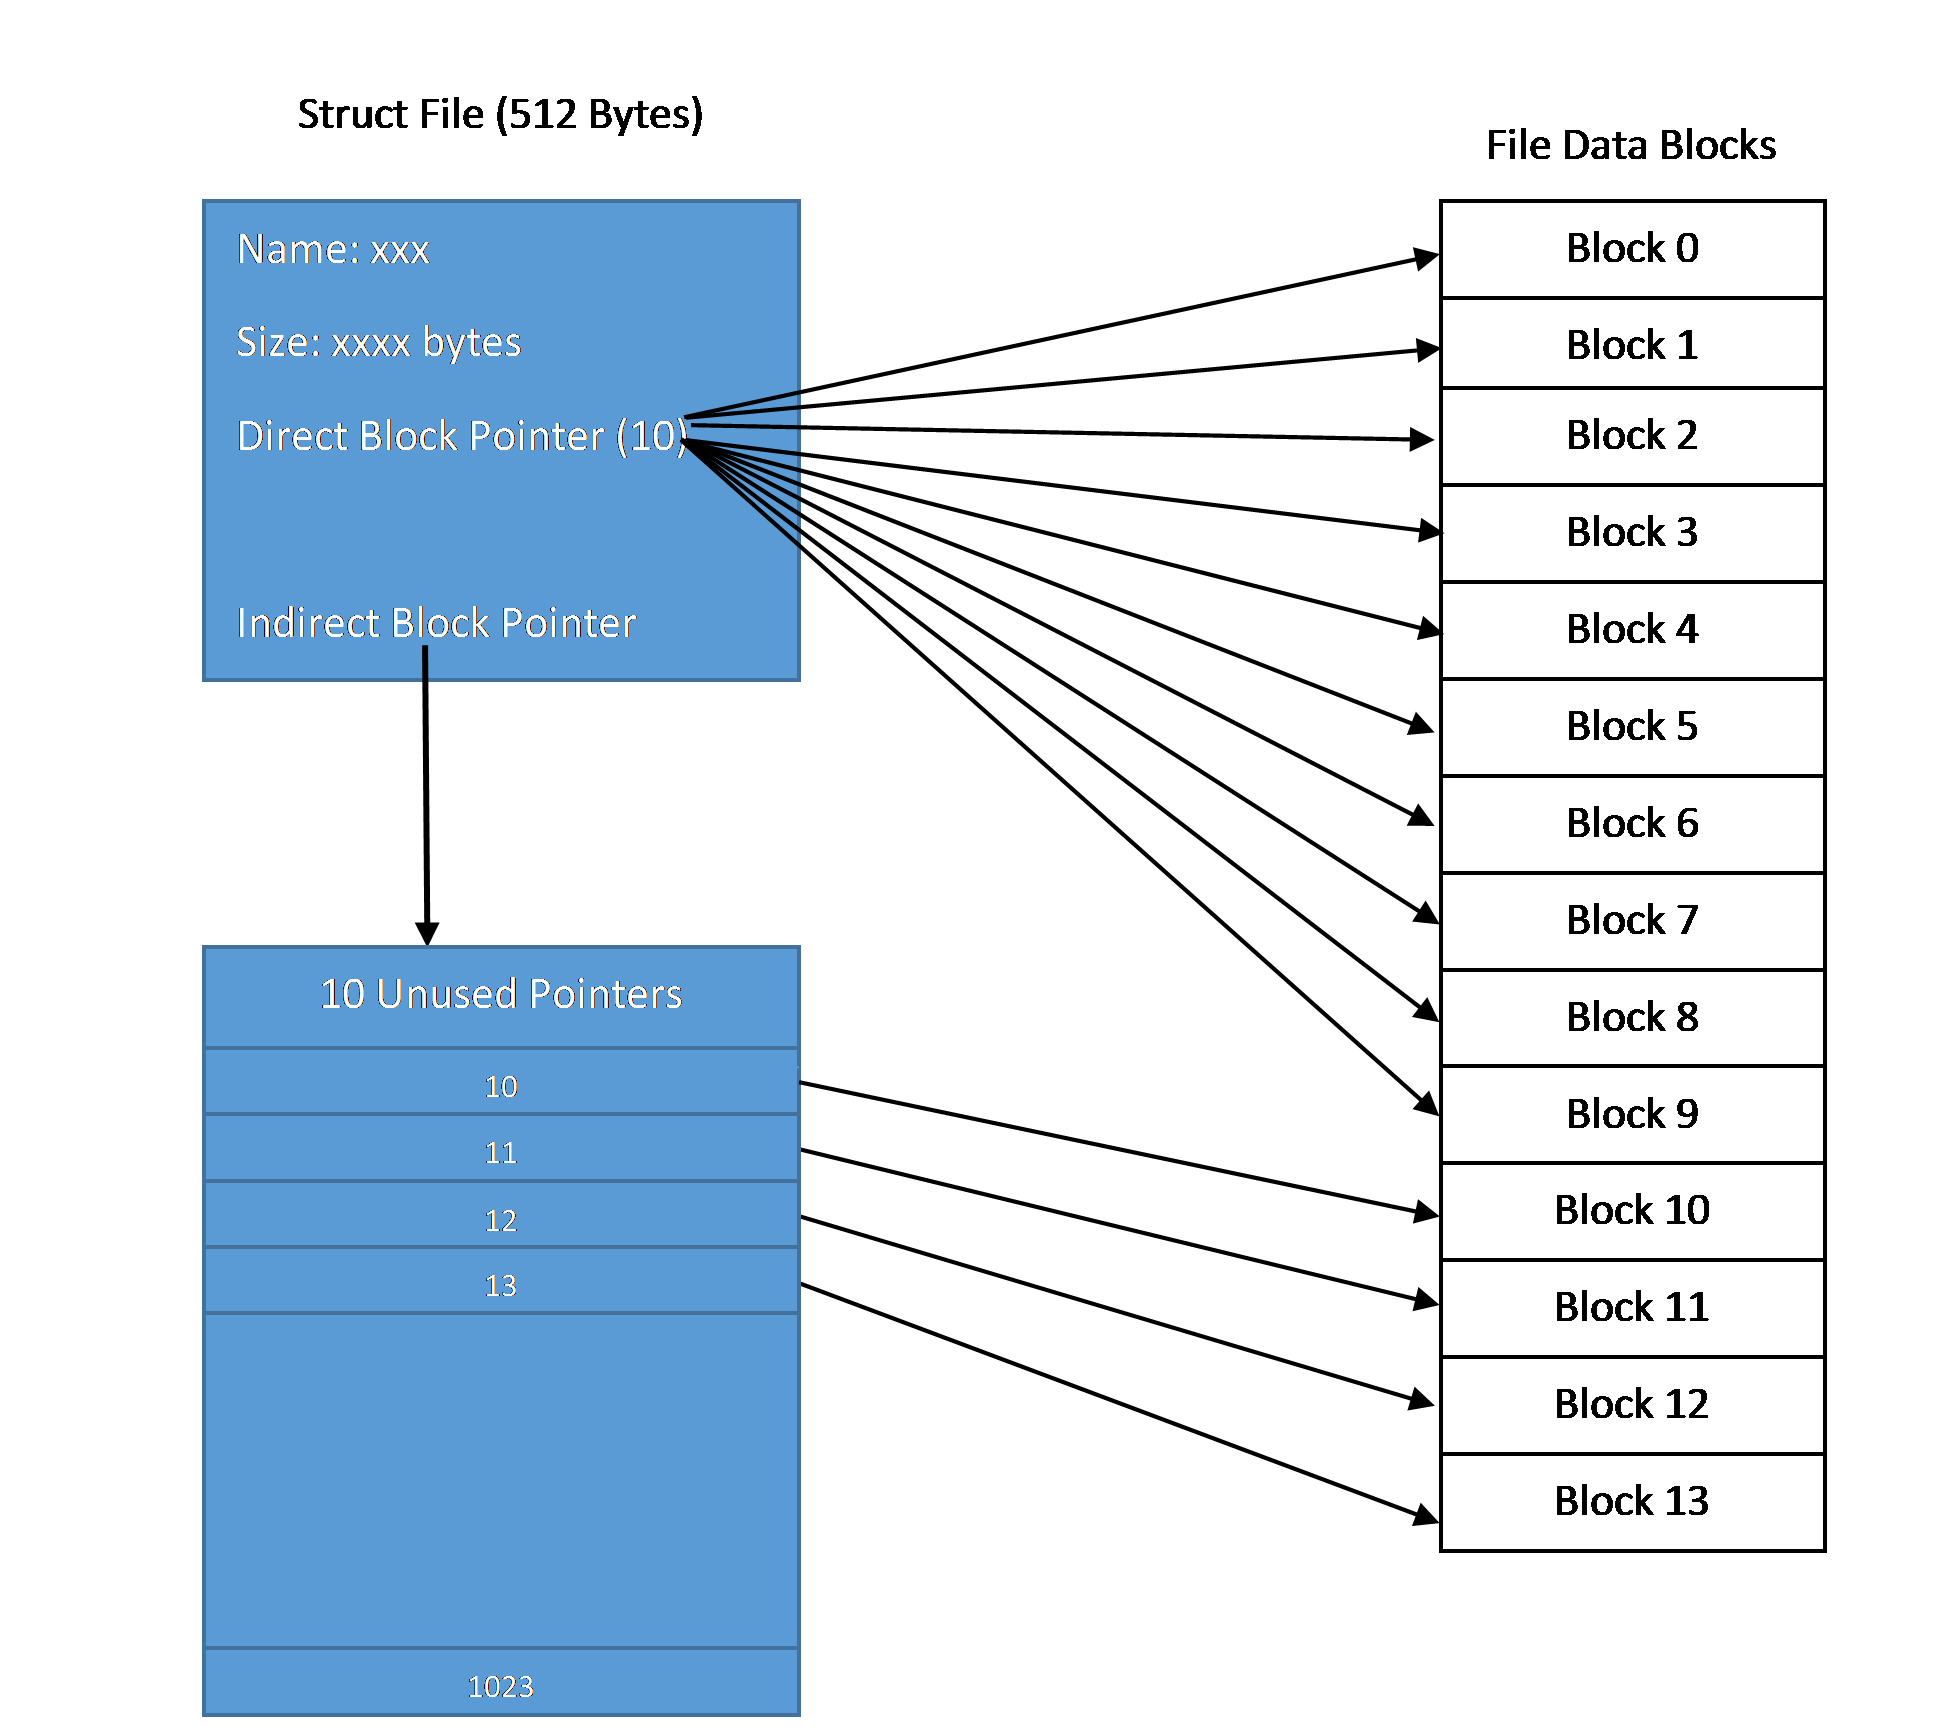
\includegraphics[width=12cm]{lab5-pic-3}
  \caption{文件控制块}\label{lab5-pic-3}
\end{figure}

对应的文件控制块的定义:

\begin{minted}[linenos]{c}
// file control blocks, defined in include/fs.h
struct File {
    u_char f_name[MAXNAMELEN];  // filename
    u_int f_size;           // file size in bytes
    u_int f_type;           // file type
    u_int f_direct[NDIRECT];
    u_int f_indirect;
    struct File *f_dir;
    u_char f_pad[BY2FILE - MAXNAMELEN - 4 - 4 - NDIRECT * 4 - 4 - 4];
};
\end{minted}

我们使用的操作系统内核中,文件名的最大长度为 MAXNAMELEN(128),每个文件控制块设有 10 个直接指针,
用来记录文件的数据块在磁盘上的位置。每个磁盘块的大小为 4KB,也就是说,这十个直接指针能够表示最大 40KB
的文件,而当文件的大小大于 40KB 时,就需要用到间接指针。
File 结构体中有一个域为 \mintinline{c}|f_indirect|,只想一个间接磁盘块,用来存储指向文件内容
的磁盘块的指针。为了简化计算,我们不使用间接磁盘块的前十个指针。文件控制块的结构如图\ref{lab5-pic-3}。

\begin{note}
我们的文件系统中文件控制块只是用了一级间接指针域,也只有一个。而在真是的文件系统中,对了支持更大的文件,通
常会使用多个间接磁盘块,或使用多级间接磁盘块。我们使用的操作系统内核在这一点上做了极大的简化。
\end{note}

\begin{thinking}\label{think-filesize}
一个 Block 最多存储 1024 个指向其他磁盘块的指针,试计算,我们的文件系统支持的单个文件的最大大小为多大?
\end{thinking}

为了更加细致地了解文件系统的内部结构,我们使用 C 语言程序(fs/fsformat.c)来模拟对磁盘的操作,掌握如何将文件
和文件夹按照文件系统的格式写入磁盘,我们也正是通过 fsformat 程序来创建一个磁盘文件 fs/fs.img 供内核使用。请
阅读 fs/fsformat.c 中的代码,掌握文件系统结构的具体细节。感兴趣的同学,可以参考 \mintinline{c}|write_file|
函数的实现,完成\mintinline{c}|write_directory| 函数,实现将一个指定目录下的文件按照目录结构写入到
fs/fs.img 的根目录下。

\section{文件系统服务}

我们实验使用的操作系统内核符合一个典型的微内核的设计,文件系统属于用户态进程,以服务的形式通过 IPC 供其他进程调用,
进行文件读写操作。具体来说,在内核开始运行时,就启动了文件系统服务进程 \mintinline{c}|ENV_CREATE(fs_serv)|,
用户进程需要进行文件操作时,使用 \mintinline{c}|ipc_send/ipc_recv| 与 \mintinline{c}|fs_serv| 进行
交互,完成操作。
在文件系统服务进程的初始化函数中,首先调用了 \mintinline{c}|serv_init| 函数准备好全局的文件打开记录表
\mintinline{c}{opentab},然后调用 \mintinline{c}|fs_init| 函数来初始化文件系统。\mintinline{c}|fs_init|
函数首先通过读取超级块的内容获知磁盘的基本信息,然后检查磁盘是否能够正常读写,最后调用 \mintinline{c}|read_bitmap|
函数检查磁盘块上的位图是否正确。执行完文件系统的初始化后,\mintinline{c}|serve| 函数被调用,文件系统服务开始运行,
等待其他程序的请求。

\begin{thinking}\label{think-fs-serve}
阅读\mintinline{c}|serve|函数的代码,我们注意到函数中包含了一个死循环\mintinline{c}|for (;;) {...}|,
为什么这段代码不会导致整个内核进入panic状态?
\end{thinking}

文件系统支持的请求类型定义在 include/fs.h 中,包含以下几种:

\begin{minted}[linenos]{c}
#define FSREQ_OPEN      1
#define FSREQ_MAP       2
#define FSREQ_SET_SIZE  3
#define FSREQ_CLOSE     4
#define FSREQ_DIRTY     5
#define FSREQ_REMOVE    6
#define FSREQ_SYNC      7
\end{minted}

用户程序在发出文件系统操作请求时,将请求的内容放在对应的结构体中进行消息的传递, \mintinline{c}|fs_serv| 进程
收到其他进行的 IPC 请求后,IPC 传递的消息包含了请求的类型和其他必要的参数,根据请求的类型执行相应的对文件系统
的操作(文件的增、删、改、查等),将结果重新通过 IPC 反馈给用户程序。

\begin{exercise}
文件 user/fsipc.c 中定义了请求文件系统时用到的 IPC 操作,user/file.c 文件中定义了用户程序读写、创建、删除
和修改文件的接口。完成 user/fsipc.c 中的 \mintinline{c}|fsipc_remove| 函数、user/file.c 中的
\mintinline{c}|remove| 函数,以及 fs/serv.c 中的 \mintinline{c}|serve_remove| 函数,实现删除指定
路径的文件的功能。
\end{exercise}

\section{正确结果展示}

在 init/init.c 中启动一个 idle 进程和文件系统服务进程:

\begin{minted}[linenos]{c}
    ENV_CREATE(user_idle);
    ENV_CREATE(fs_serv);
\end{minted}

就能开始对文件系统的检测,运行文件系统服务,等待应用程序的请求。

\begin{minted}[linenos]{c}
FS is running
FS can do I/O
superblock is good
diskno: 0
diskno: 0
read_bitmap is good
diskno: 0
alloc_block is good
file_open is good
file_get_block is good
file_flush is good
file_truncate is good
diskno: 0
file rewrite is good
\end{minted}

\section{实验思考}

\begin{itemize}
\item \hyperref[think-proc]{\textbf{\textcolor{baseB}{Unix /proc 文件系统}}}
\item \hyperref[think-disksize]{\textbf{\textcolor{baseB}{磁盘最大体积}}}
\item \hyperref[think-filesize]{\textbf{\textcolor{baseB}{文件系统支持的单个文件的最大体积}}}
\item \hyperref[think-fs-serve]{\textbf{\textcolor{baseB}{文件系统服务进程运行机制}}}
\end{itemize}

\section{实验挑战}




